% -*- root: ../cnf-json.tex -*-

Semi-structured formats like \json allow users to design schemas on-the-fly, as data is generated.
For example, adding a new attribute to the output of a system logger does not break backwards compatibility with existing data.
This flexibility facilitates the addition of new features and enables low-overhead adaptation of data-generating processes.
However, because the data does not have a consistent underlying schema, it can be harder (and slower) to explore than simple tabular data.
The logic of each and every query must explicitly account for variations in the schema like missing attributes.  
Performance also suffers, as there is no one physical data representation that is ideal for all schemas.

To address these problems, a variety of techniques~\cite{DBLP:conf/cidr/LiuG15,DBLP:conf/edbt/BaaziziLCGS17,DBLP:conf/sigmod/DiScalaA16,DBLP:conf/vldb/GoldmanW97,spoth:2017:cidr:adaptive} have arisen to generate schemas after-the-fact.
The goal of these \emph{semi-structured schema discovery} (\sssd) techniques is to propose a schema for collections of \json records.
A common approach to this problem is to bind the \json records to a normalized relational representation, or in other words, to derive a set of flat \emph{views} over the hierarchical \json data.

Existing automated approaches to this problem (e.g., \cite{DBLP:conf/sigmod/DiScalaA16,DBLP:conf/vldb/GoldmanW97}) operate in a single-pass: They propose a schema and consider their job done.
Unfortunately these techniques also rely heavily on general heuristics to select from among a set of schema design choices, as a clear declarative specification of a domain would be tantamount to having the schema already.
To supplement domain-agnostic heuristics with feedback from domain experts, we propose a new \emph{iterative and interactive} approach to \sssd called \systemnametwo.

\systemnametwo provides a OLAP-style interface (with analogs to roll-up, drill-down, and slice+dice) specialized for exploring collections of \json records.  
Every state of this interface corresponds to a relational view defined over the \json data.
When ready, this view can be exported to a classical RDBMS or similar tool for simplified, more efficient data access.
In this paper, we explore several design options for \systemnametwo, and discuss how each interacts with the challenges of \sssd.

\subsection{Extracting Relational Entities}
The first class of challenges we address involve the nuts and bolts of mapping hierarchical \json schemas to flat relational entities.  
Fundamentally, this involves a combination of three relational operators: Projection, Selection, and Unnesting.  

\tinysection{Projecting Attributes}
\json schema discovery can, naively, be thought of as a form of schema normalization~\cite{Codd:1979:EDR:320107.320109}, where each distinct path in a record is treated as its own attribute.
Entities then, are simply groups of attributes projected out of the \json data, and 
the \sssd problem reduces to finding such groups (e.g., by using Functional Dependencies~\cite{DBLP:conf/sigmod/DiScalaA16}).  

\tinysection{Selecting Records}
This naive approach fails in situations where the collection of \json records is a mix of different entity types that share properties.
As a simple example, Twitter streams mix three entity types: tweets, retweets, and deleted tweets.  
Although each entity appears in distinct records, they share attributes in common.
Hence, entity extraction is not just normalization in the classical sense of partitioning attributes, but rather also a matter of partitioning records by content.

\tinysection{Collapsing Nested Collections}
\json specifies two collection types: Arrays and Objects.  
Typically the former is used for encoding nested collections and the latter for encoding tuples with named attributes.
However, this is not a strict requirement.
For example, latitude and longitude are often encoded as a 2-element array.
Conversely, in some data sets, objects are used as way to index collections by named keys rather than by positions.
Hence, simple type analysis can not distinguish between the two cases.
This is problematic because treating a collection as a tuple creates an explosion of attributes that make classical normalization techniques incredibly expensive.

\subsection{Human-Scale \sssd}
Even in settings where \json data is comparatively well behaved, it is common for it to have dozens, or even hundreds of attributes per record.  
Similarly, individual \json records can be built from any of the hundreds or thousands (or more) different permutations of the full set of attributes used across the entire collection.
Bringing this information down to human scale requires simultaneously simplifying and summarizing.

\tinysection{Summarization}
For the purposes of entity construction, the full set of attributes is often unnecessary.
It is often possible to collapse multiple attributes together, or express attributes as equivalent alternatives.
As an example, an address might consist of four distinct attributes city, zip code, street, and number when it could conceptually be expressed as just one.

\tinysection{Visualization}
In addition to simplifying the underlying problem, it is also useful to give users a coarse ``top-down'' view of the schema process.
Specifically, users need to (1) be able to see patterns of structural similarity between distinct schemas, and (2) understand how much variation exists in the data set as-is.

\tinysection{Iteration}
By combining straightforward summarization and data visualization techniques, \systemnametwo helps users to quickly identify natural clusters of records and attributes that represent relational entities.
\systemnametwo facilitates an \emph{iterative} schema design process to allow human experts to better evaluate whether structures in the data indicate conceptual relationships between records or attributes, or are merely data artifacts.

\begin{figure}
\centering
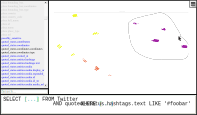
\includegraphics[width=0.9\linewidth]{SchemaSummarization/img/UI}
\caption{Prototype user interface for \systemnametwo.}
\label{fig:ui}
\end{figure}

\subsection{Overview}
Figure~\ref{fig:ui} shows the prototype interface of \systemnametwo. 
The pane on the left, discussed in Section~\ref{sec:distribution}, shows the schema of the currently selected JSON view, highlighting attributes and groups based on relevance.
The pane on the right, discussed in Section~\ref{sec:visualization}, provides a top-down visual sketch of schemas in the currently selected JSON data, and allows users to interactively filter out parts of it.
Finally in Section~\ref{sec:visualization}, we show examples of how \systemnametwo facilitates incremental, iterative exploration and mapping of JSON schemas.




